\documentclass{article}

\usepackage{polski}
\usepackage[UTF8]{inputenc}
\usepackage{graphicx}
\usepackage{float}
\usepackage[margin=1in]{geometry}
\usepackage{graphicx}
\usepackage{amsmath}
\usepackage{mathtools}
\usepackage{amssymb}
\usepackage{multirow}
\usepackage{changepage}


\title{Sprawozdanie}
\begin{document}

\begin{center}
\bgroup
\def\arraystretch{1.5}
\begin{tabular}{|c|c|c|c|c|c|}
	\hline
	EAIiIB & \multicolumn{2}{|c|}{\begin{tabular}{@{}c@{}}Autor 1 \\ Autor 2\end{tabular}} & Rok II & Grupa 5 & Zespół 6 \\
	\hline
	\multicolumn{3}{|c|}{\begin{tabular}{c}Temat: \\ Mostek Wheatstone'a \end{tabular}} & 
	\multicolumn{3}{|c|}{\begin{tabular}{c}Numer ćwiczenia: \\ 32 \end{tabular}} \\
	\hline
	Data wykonania & Data oddania & Zwrot do poprawki & Data oddania & Data zaliczenia & Ocena \\[8ex]
	\hline
\end{tabular}
\egroup
\end{center} 

%WSTEP
\section{Cel ćwiczenia}
Praktyczne zastosowanie praw Kirchhoffa, sprawdzenie zależności określających opór zastępczy dla połączenia szeregowego i równoległego.

\section{Wstęp teoretyczny}
\subsection{Pierwsze prawo Kirchhofa}
Suma natężeń prądów wpływających do rozgałęzienia, równa jest sumie natężeń prądów wypływających z tego rozgałęzienia.
\subsection{Drugie prawo Kirchhofa}
W obwodzie zamkniętym suma spadków napięć na wszystkich odbiornikach prądu musi być równa sumie napięć na źródłach napięcia.
\subsection{Prawo Ohma}
Natężenie prądu stałego $I$ jest proporcjonalne do całkowitej siły elektromotorycznej w obwodzie zamkniętym lub do różnicy potencjałów (napięcia elektrycznego) między końcami części obwodu nie zawierającej źródeł siły elektromotorycznej
\subsection{Rezystancja}
R jest to trudność na jaką napotykają przemieszczające się elektrony. Rezystancja przewodu zależy od długości (do której jest wprost proporcjonalna), od pola przekroju poprzecznego (do którego jest odwrotnie proporcjonalna) oraz od materiału z którego przewód został wykonany.
\subsection{Natęzenie prądu}
Jest wielkością fizyczną charakteryzującą przepływ prądu elektrycznego zdefiniowaną jako stosunek wartości ładunku elektrycznego przepływającego przez wyznaczoną powierzchnię do czasu przepływu ładunku.
$$ I = \frac{\partial Q}{\partial t} $$
\subsection{Napięcie elektryczne}
Różnica potencjałów elektrycznych między dwoma punktami obwodu elektrycznego lub pola elektrycznego. Napięcie elektryczne to stosunek pracy wykonanej podczas przenoszenia ładunku między punktami, dla których określa się napięcie do wartości tego ładunku.
$$ U_{AB} = \frac{W_{A\rightarrow B}}{q}$$
\section{Ukłąd pomiarowy}
Zestaw ćwiczeniowy stanowi mostek Wheatstone'a, w skład obwodu wchodzą:
\begin{enumerate}
\item Listwa z drutem oporowym, zaopatrzona w podziałkę milimetrową i kontakt ślizgowy, umożliwiający zmiany długości odcinków a i b.
\item Opornica dekadowa $R_{2}$
\item Symbolem $R_{x}$ oznaczono zestaw oporników wmonotowanych na odpowiedniej płytce z pleksiglasu.
\item Mikroamperomierz G jako wskaźnik zerowania mostka.
\item Zasilacz
\end{enumerate}
\begin{figure}[!htb]
	\centering
	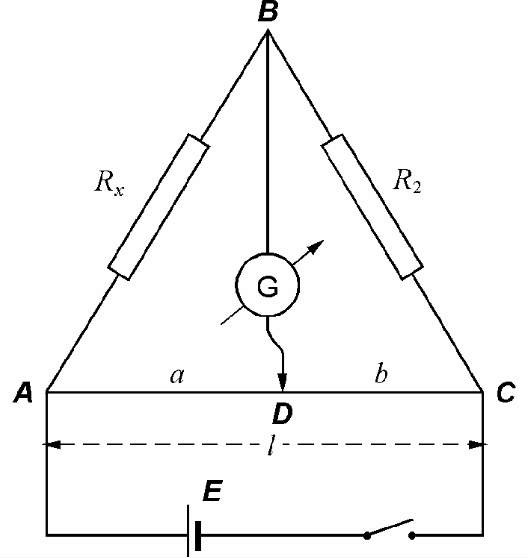
\includegraphics[scale=0.5]{mostek.png}
	\caption{Schemat elektryczny mostka}
\end{figure}	
\section{Wykonanie ćwiczenia}
\begin{enumerate}
	\item Podłączenie obwodu elektrycznego według schematu.
	\item Wykonano po 10 pomiarów oporów przy różnych oporach wzorcowych dla oporów $R_{1}$,$R_{2}$.
	\item Wykonano analogiczne pomiary dla połączenia równoległego i szeregowego tych oporników.
\end{enumerate}
	

%KONIEC WSTEPU	
\pagebreak
\section{Opracowanie wyników}
\subsection{Obliczenia}
\begin{enumerate}
	\item Wyznaczamy wartość nieznanych oporów ze wzoru:
	$$ R_{x} = R_{w}\frac{a}{l_{0}-a} $$
	\item Obliczamy wartość średnią dla każdego oporu z punktu 1 oraz jej niepewność pomiarową.
	$$ \overline{R} = \dfrac{1}{n}\sum_{i=1}^{n} R_{x_{i}} $$
	$$ u(R_{x}) = \sqrt{\frac{\sum_{i=1}^{n}(R_{i}-\overline{R_{x}})^2}{n(n-1)}}$$
	\item Wyznaczamy analogicznie wartość oporów dla połączenia szeregowego i równoległego.
	\item Wyznaczamy wartość oporu zastępczego dla połączenia szeregowego:
	$$ R_{s} = R_{x1}+R_{x2} $$
Niepewność z prawa przenoszenia niepewności pomiarowych:
$$ u(R_{s}) = \sqrt{\bigg(\frac{\partial R_{s}}{\partial R_{1}}u(R_{1})\bigg)^2+\bigg(\frac{\partial R_{s}}{\partial R_{2}}u(R_{2})\bigg)^2} = \sqrt{u(R_{1})^2+u(R_{2})^2}$$	
	
	\item Wyznaczamy wartość oporu zastępczego dla połączenia równoległego:
	$$ \frac{1}{R_{r}}=\frac{1}{R_{1}}+\frac{1}{R_{2}}=\frac{R_{1}R_{2}}{R_{1}+R_{2}}$$
Niepewność z prawa przenoszenia niepewności pomiarowych:
$$ u(R_{r}) = \sqrt{\bigg(\frac{\partial R_{s}}{\partial R_{1}}u(R_{1})\bigg)^2+\bigg(\frac{\partial R_{s}}{\partial R_{2}}u(R_{2})\bigg)^2} = \sqrt{\bigg(\frac{R_{2}^2}{(R_{1}+R_{2})^2}u(R_{1})\bigg)^2+\bigg(\frac{R_{1}^2}{(R_{1}+R_{2})^2}u(R_{2})\bigg)^2}$$	
\end{enumerate}
\begin {table}[H]
\caption {Wyniki obliczeń} \label{tab:title}
\begin{center}
\def\arraystretch{1.3}
	\begin{tabular}{|c|c|c|c|c|}
		\hline
		& \begin{tabular}{c} $R_{s}$ wyznaczone  \\ \mbox{[$\Omega$]}  \end{tabular}  & 
		 \begin{tabular}{c}	$R_{s}$ obliczone \\ \mbox{[$\Omega$]}  \end{tabular} &
		 \begin{tabular}{c} $R_{r}$ wyznaczone \\ \mbox{[$\Omega$]}  \end{tabular} &
		 \begin{tabular}{c} $R_{r}$ obliczone \\ \mbox{[$\Omega$]} \end{tabular} \\ 
		\hline
		Średnia wartość & $28,195$ & $27,984$ & $6,288$ & $ 6,277$\\
		\hline
		Niepewność & $0,0819$ & $0,0829$ & $0,0478$ & $0,0257$\\
		\hline
	\end{tabular}

\end{center}
\end{table}

\pagebreak
\subsection{Obliczenie niepewności rozszerzonej dla połączenia szeregowego}
\label{s1}
$k = 2$ \\
\begin{equation*}
\begin{aligned}
& |R_{wyznaczone} - R_{obliczone}| = 28,195  [\Omega] - 27,984  [\Omega] = 0,211 [\Omega] \\
& U(R_{wyznaczone} - R_{obliczone}) = k \cdot \sqrt{u(R_{wyznaczone})^2 +u(R_{obliczone})^2} = 0,233  [\Omega]\\
& |R_{wyznaczone} - R_{obliczone}| < U(R_{wyznaczone} - R_{obliczone}) \\
\end{aligned}
\phantom{\hspace{8cm}} %%<---adjust the value as you want
\end{equation*}
\\~\\
\noindent
Wartość wyznaczona zastępczego oporu jest zgodna z wartością obliczoną.
\subsection{Obliczenie niepewności rozszerzonej dla połączenia równoległego}
\label{s2}
$k = 2$ \\
\begin{equation*}
\begin{aligned}
& |R_{wyznaczone} - R_{obliczone}| = 6,288  [\Omega] - 6,277  [\Omega] = 0,011 [\Omega] \\
& U(R_{wyznaczone} - R_{obliczone}) = k \cdot \sqrt{u(R_{wyznaczone})^2 +u(R_{obliczone})^2} = 0,108  [\Omega]\\
& |R_{wyznaczone} - R_{obliczone}| < U(R_{wyznaczone} - R_{obliczone})
\end{aligned}
\phantom{\hspace{8cm}} %%<---adjust the value as you want
\end{equation*}
\\~\\
\noindent
Wartość wyznaczona zastępczego oporu jest zgodna z wartością obliczoną.


 \section{Wnioski}
	Korzystając z mostka Wheatstone’a wyznaczyliśmy nieznane wartości oporników oraz opory zastępcze gdy zostały one połączone szeregowo oraz równolegle. Niepewności uzyskane przy pomiarze rezystancji każdego opornika oraz przy połączeniu ich równolegle i szeregowo są zadowalająco małe, a tym samym wyznaczone opory są precyzyjne. 
	\\ \\
	Zmierzona wartość rezystancji oporników  $R_{1}$ i $R_{2}$ połączonych szeregowo oraz równolegle jest zgodna z wartościami obliczonymi (\ref{s1} i \ref{s2}). W związku z czym możemy stwierdzić, że wzory do obliczenia oporu zastępczego dla połączeń równoległych i szeregowych są prawdziwe.
	
\end{document}